\documentclass{article}
\usepackage{graphicx} % Inserting graphics (\includegraphics{<graphic>}) https://www.overleaf.com/learn/latex/Inserting_Images
\usepackage{amssymb,amsmath,amsthm} % Math symbols, enviroments and more
\usepackage{xcolor} % Changing text color (\textcolor{<color>}{<text>}) https://www.overleaf.com/learn/latex/Using_colours_in_LaTeX
\usepackage{float} % Provides H specifier for floats
\usepackage[output-decimal-marker=\text{,}, exponent-product=\ensuremath{\cdot}, range-phrase={ - }]{siunitx} % SI units with correct number formatting (\num{<value>}, \si{<unit>}, \SI{<value>}{<unit>})
\usepackage{hyperref} % Hyperlinks (\href{<url>}{<text>}, \url{<url>}) https://www.overleaf.com/learn/latex/Hyperlinks
\usepackage{pgf} % Graphics https://www.overleaf.com/learn/latex/TikZ_package
\usepackage[siunitx, RPvoltages, european]{circuitikz} % Drawing circuits https://www.overleaf.com/learn/latex/CircuiTikz_package
\usepackage{multicol} % Allows merging multiple cells in one table row (\multicolumn{<number of columns>}{<style eg. |c>}{<content>})
\usepackage{multirow} % Merging multiple cells in one table column (\multirow{<number of rows>}{<width eg. * for natural width>}{<content>}
\usepackage{pgfplots} % Data plots https://www.overleaf.com/learn/latex/Pgfplots_package
\pgfplotsset{compat=1.18} 
\usepackage{pdfpages} % Allows inserting a pdf page (\includepdf[pages=<which pages, - for all>]{<filename>})
\usepackage[a4paper, margin=1in]{geometry} % Sets paper size to A4 with content no bigger than 6 by 8 inch https://www.overleaf.com/learn/latex/Page_size_and_margins
\usepgfplotslibrary{polar}
\usepackage{csvsimple} % Creating tables based on CSV's
\usepackage{lscape} % Landscape pages (\begin{landscape})
\usetikzlibrary{external} % Caching images
\tikzexternalize[prefix=tikz/] % Caching images
\usepackage{subfig}  % Multiple figures in a row
\DeclareSIUnit\torr{Torr}
\usepackage{rotating}
\usepackage{pdflscape}

\title{Ion Gauge Controller}
\author{Jakub Jendryka}
\date{22.10.2023}

\begin{document}
\maketitle

\section{Introduction}
This project is a Bayard-Alpert vacuum gauge controller designed to work within the EuroMeasure system.
\subsection{Bayard-Alpert gauge}
Bayard-Alpert gauge is a type of a vacuum gauge that uses gas ionization through electron impact as a way
to measure high vacuums in the range of \SI{1e-3}{Torr} - \SI{1e-10}{Torr} or \SI{1e-1}{\pascal} - \SI{1e-8}{\pascal}.
Electrons are boiled-off from the cathode which is a tungsten filament heated with a current passed through it.
Electrons are then accelerated using a grid at a strong positive potential.
Accelerated electrons going through the vacuum have a chance to struck a residual gas molecule and ionise it.
This, now positively charged, ion is attracted by the anode at a slight negative potential.
Current that flows into the anode due to those ions is therefore proportional to the pressure inside the gauge.

\begin{figure}[H]
	\begin{center}
		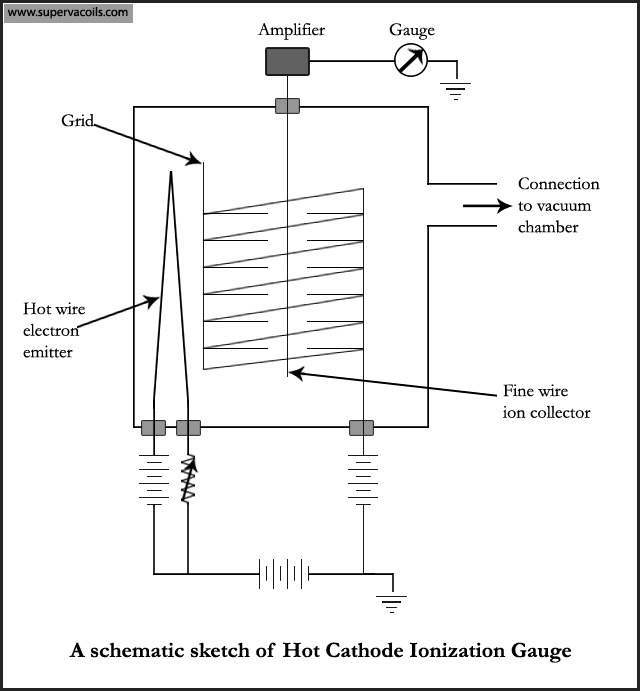
\includegraphics[width=0.5\textwidth]{figures/ion_gauge.jpg}
	\end{center}
	\caption{Hot ionisation vacuum gauge diagram}
	\label{fig:ion_gauge}
	% https://www.supervacoils.com/vacuum-gauges-explained/hot-ionization-gauge/
\end{figure}


\subsection{EuroMeasure}
EuroMeasure is a mechanical, electronic and protocol standard for measurement and control systems.
It is developed at Wrocław University of Science and Technology faculty of Microsystems. This standard defines a module that can be connected with others on a single bus.
It was designed to be compatible with standard Eurocard enclousures as well as to be cheap to manufacture.
Each module consists of one or more PCB's, each taking up one module width. Each PCB can be connected to a backplane using two IDC10 connectors providing power and control signals and can also have an additional debug connector.
Additional connectors and other parts needed for operation can be mounted on the module front panel, which is attached to the PCB's.

\section{Requirements}
From the theory of operation of the vacuum gauge arise several requirements. The controller needs to heat the cathode, polarize all the electrodes in relation to each other and measure currents flowing in and out of the electrodes.
This device is expected to operate with SJ2 vacuum gauge. Gauge parameters per its datasheet are as follows:
\begin{itemize}
	\item Cathode current: \SI{1.5}{\ampere}$\pm$\SI{0.1}{\ampere}
	\item Cathode emission current: \SI{5}{\milli\ampere}
	\item Grid voltage: \SI{200}{\volt}
	\item Anode voltage: \SI{-25}{\volt}
	\item Sensitivity: \SI{16}{\frac{\milli\ampere}{\milli\ampere\cdot\torr}}
	\item Working range: \SIrange{1e-7}{1e-3}{\torr}
\end{itemize}

It is expected that cathode current is adjusted to stabilize electron emission current at the required level.
Using working range, emission current and sensitivity, anode current range can be calculated to be around: \SI{10}{\nano\ampere} - \SI{100}{\micro\ampere}.
Cathode voltage at specified current was measured to be around \SI{8}{\volt}.
In summary the device needs to supply continously adjustable cathode current, polarize the grid and measure grid current, polarize the anode and measure anode current.
It would be beneficial if parameters of the device were adjustable, as most Bayard-Alpert gauges have similar requirements and this would allow to support other models.

As the device is going to be a part of EuroMeasure system it needs to conform to its specification.
It is expected that it will take up one module width, therefore it should consist of one \num{10}$\times$\SI{10}{\centi\meter} PCB with max
component height of \SI{16}{\milli\meter} at the top and \SI{2}{\milli\meter} at the bottom. There are four M3 mounting holes at the corners of the PCB, \SI{5}{\milli\meter} from the edge.
There are three right-angle IDC10 connectors at the back edge of the board. One for power ($\pm$\SI{15}{\volt} and $+$\SI{5}{\volt}), one for data (I2C communication and high voltage lockout) and one for debugging (SWD and UART).
Connector for the vacuum gauge should be mounted to the front panel. The device is expected to operate in standard laboratory conditions.
It should emit as little as possible EMI, and should not backfeed noise onto $\pm$\SI{15}{\volt} power supply rails and should disable hazardous voltages when lockout line is not energized.

\section{Design}

Block diagram of the design is presented in figure \ref{fig:block_diagram}. It also serves as top level schematic sheet.
Starting with the gauge it is connected to the controller using a single connector. Each of the electrodes is supplied by a separate switchmode power supply.
Anode and grid power supplies are constant voltage, not controllable power supplies with galvanicly isolated output. This allows for easy current measurement on the low side of the supply.
Cathode supply is programmable constant voltage switchmode supply. Using current measurement data from the grid, microcontroller can modify output voltage to stabilize emission current at required level.
To allow for cathode health monitoring, its voltage as well as current are monitored.
As cathode response is not very fast due to its thermal mass it was decided to use a fully digital control loop, as it will be easier to implement and add cathode safety features that disallow accidental cathode burnout.
Every important parameter is digitized in the ADC block and processed by the microcontroller. Power and interface are connected through the backplane connector.
To minimize backfed noise, voltages suppling power supplies are filtered.

\begin{landscape}
	\begin{figure}
		\begin{center}
			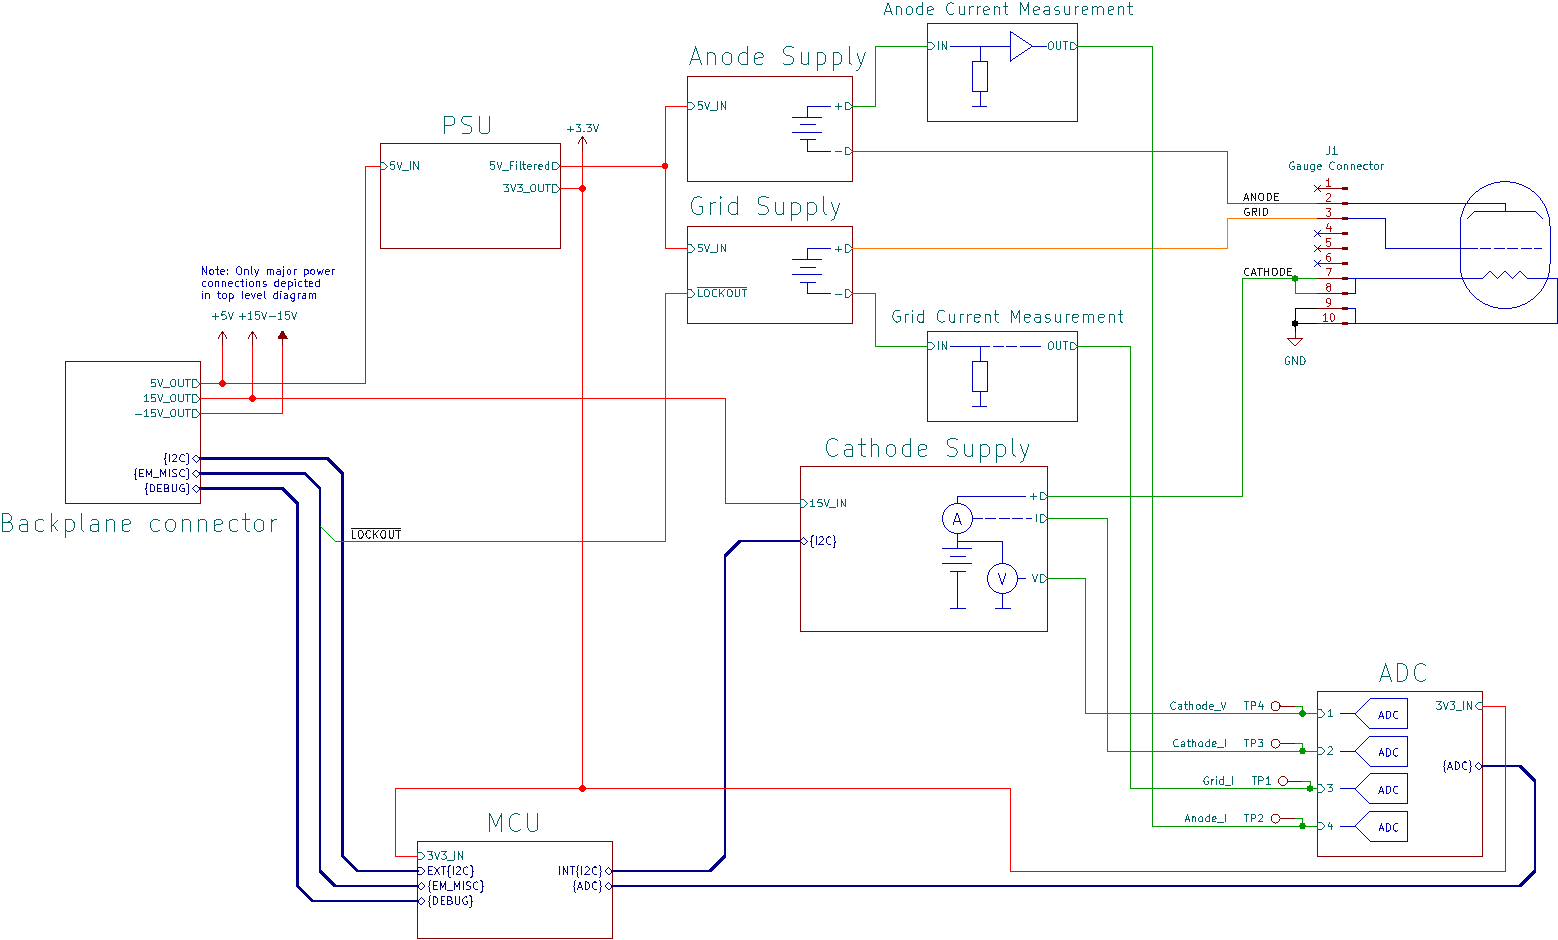
\includegraphics[width=1.5\textwidth]{figures/block_diagram.pdf}
		\end{center}
		\caption{Block diagram}\label{fig:block_diagram}
	\end{figure}
\end{landscape}



\subsection{Anode supply}
To generate anode voltage SN6507 push-pull transformer driver was selected. It was already tested in a previous project and offered required low-noise operation due to configurable slew rate.
To pair with the driver 750316856 transformer was selected. It offered high enough turn ratio of \num{4.67} (It was decided to set this voltage pretty high to be able to modify output voltage in the future).
Output voltage was calculated using equation \ref{eq:anode_dcdc_voltage}:
\begin{equation}
	V_{out} = 2\cdot V_{in} \cdot n_{ratio}  = 2 \cdot \SI{5}{\volt} \cdot \num{4.67} = \SI{46.7}{\volt}
	\label{eq:anode_dcdc_voltage}
\end{equation}
To not saturate the core, sufficiently high switching voltage is required. Manufacturer specifies transformer "voltage-time" to be \SI{15}{\volt\micro\second}.
Minimum frequency is calculated using equation \ref{eq:transformer_saturation}.
\begin{equation}
	F_{min} = \frac{V_{in}}{VT} = \frac{\SI{5}{\volt}}{\SI{15}{\volt\micro\second}} = \SI{333}{\kilo\hertz}
	\label{eq:transformer_saturation}
\end{equation}
To have sufficient margin operating frequency was set to \SI{500}{\kilo\hertz}. To do this, resistor R16 was set to \SI{22}{\kilo\ohm} in accordance to the specification.
Programmable current limit was set to \SI{500}{\milli\ampere} with R22, and soft start time was set to \SI{3.8}{\milli\second} according to equation \ref{eq:anode_soft_start}.
\begin{equation}
	T_{ss} = \frac{C_{17}}{\SI{275}{\micro\ampere}-\frac{0.6}{R_{17}}} = \SI{3.8}{\milli\second}
	\label{eq:anode_soft_start}
\end{equation}
Undervoltage lockout was set to be around \SI{3.8}{\volt} (eq. \ref{eq:anode_undervoltage}).
\begin{equation}
	U_{UVLO} = \SI{1.5}{\volt} \cdot \left(1+\frac{R_{19}}{R_{15}}\right) = \SI{3.8}{\volt}
	\label{eq:anode_undervoltage}
\end{equation}

Voltage from the transformer is rectified with a full bridge rectifier build using "low-emission" PMEG200G20 diodes. Their low forward voltage and reverse charge limit switching noise.
Voltage is then filtered using capacitors and an inductor. LTSpice simulations show around \SI{-75}{\deci\bel} damping at switching frequency. It is very important to take into account capacitor derating due to DC bias.
To further reduce noise and stabilize voltage level, an adjustable voltage regulator is used.
It's output voltage is set using R22 and R22 according to the equation \ref{eq:anode_output_voltage}. Diodes D12 and D13 are added for IC protection from capacitor discharge, following manufacurer recommendation.
\begin{equation}
	V_{out}= \SI{1.25}{\volt}\cdot\left(1+\frac{R_{22}}{R_{21}}\right) + \SI{50}{\micro\ampere}\cdot R_{22}
	\label{eq:anode_output_voltage}
\end{equation}

\includepdf[landscape=true, pages=4]{figures/schematic.pdf}

\section{Anode current measurement}
Anode current measurement is the most critical measurement in the whole device. Due to this extra care must be taken. Transimpedance amplifier configuration was considered, however stability concerns dictated the change to the current configuration.
Anode current is measured using R41 \SI{1}{\kilo\ohm} resistor. This gives voltage of \SI{0.1}{\volt} for full range of \SI{100}{\micro\ampere}. This voltage shift should not influence the measurement significantly as it is only a \SI{0.4}{\%} change.
Due to voltage in the low measurement range being only \SI{10}{\micro\volt} a low offset precision op-amp is needed for amplification of the signal.
OPA2187 was selected as it specifies low offset voltage of \SI{10}{\micro\volt} with drift of only \SI{0.001}{\micro\volt/\kelvin} and bias current of \SI{100}{\pico\ampere}.
It is used to provide a gain of x11 to more fully utilise ADC range. Diode DZ3 is added for ADC protection.
\includepdf[landscape=true, pages=7]{figures/schematic.pdf}

\end{document}
